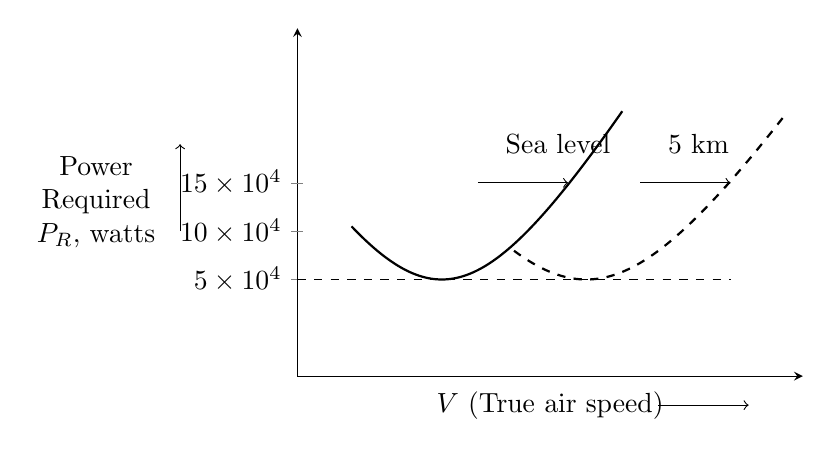
\begin{tikzpicture}
    \begin{axis}[
        width=8cm, height=6cm, % Adjusted size for a more compact graph
        xmin=0, xmax=1.4,
        ymin=0, ymax=1.8,
        axis lines=left,
        xlabel={$V$ (True air speed)},
        ylabel={Power\\Required\\$P_R$, watts},
        ylabel style={rotate=-90, align=center},
        xtick=\empty, ytick=\empty,
        extra y ticks={0.5, 0.75, 1},
        extra y tick labels={$5 \times 10^4$, $10 \times 10^4$, $15 \times 10^4$},
        extra x ticks={},
        clip=false
    ]
    
    % Sea level curve (solid line with dip)
    \addplot[
        domain=0.15:0.9,
        samples=100,
        thick
    ]
    {(1+(10*(x-0.4)^2))^(0.5)-0.5}; % Adjusted formula for a more pronounced dip and rise
    \node[right] at (axis cs:0.55,1.2) {Sea level};
    
\draw[->] (0.5,1) -- ++(0.25,0) node[right] {};
\draw[->] (0.95,1) -- ++(0.25,0) node[right] {};
\draw[->] (1,-0.15) -- ++(0.25,0) node[right] {};
\draw[->] (-0.325,0.75) -- ++(0,0.45) node[right]{} ;
    % 5 km curve (dashed line with similar shape but slightly higher)
    \addplot[
        domain=0.6:1.35,
        samples=100,
        thick,
        dashed
    ]
    {(1+(8*(x-0.8)^2))^(0.5)-0.5}; % Adjusted formula for 5 km
    \node[right] at (axis cs:1,1.2) {5 km};

    % Dashed horizontal line at y=0.5
    \draw[dashed] (axis cs:0,0.5) -- (axis cs:1.2,0.5);

    \end{axis}
\end{tikzpicture}

